\pagelayout{wide} % No margins
\addpart{Introduction}
\pagelayout{margin} % Restore margins

\setchapterpreamble[u]{\margintoc}
\chapter{Context and motivation}
\labch{intro:context}

\blindtext\blindtext\blindtext\blindtext\blindtext
\begin{marginfigure}[-5.5cm]
    \includegraphics[]{figures/shareholders-driven-apocalysis.png}
    \caption{``Yes, the planet got destroyed. But for a beautiful moment in time, we created a lot of value for shareholders''}
    % \labfig{}
\end{marginfigure}


\blindtext\blindtext\blindtext\blindtext


\begin{figure}[htbp]
    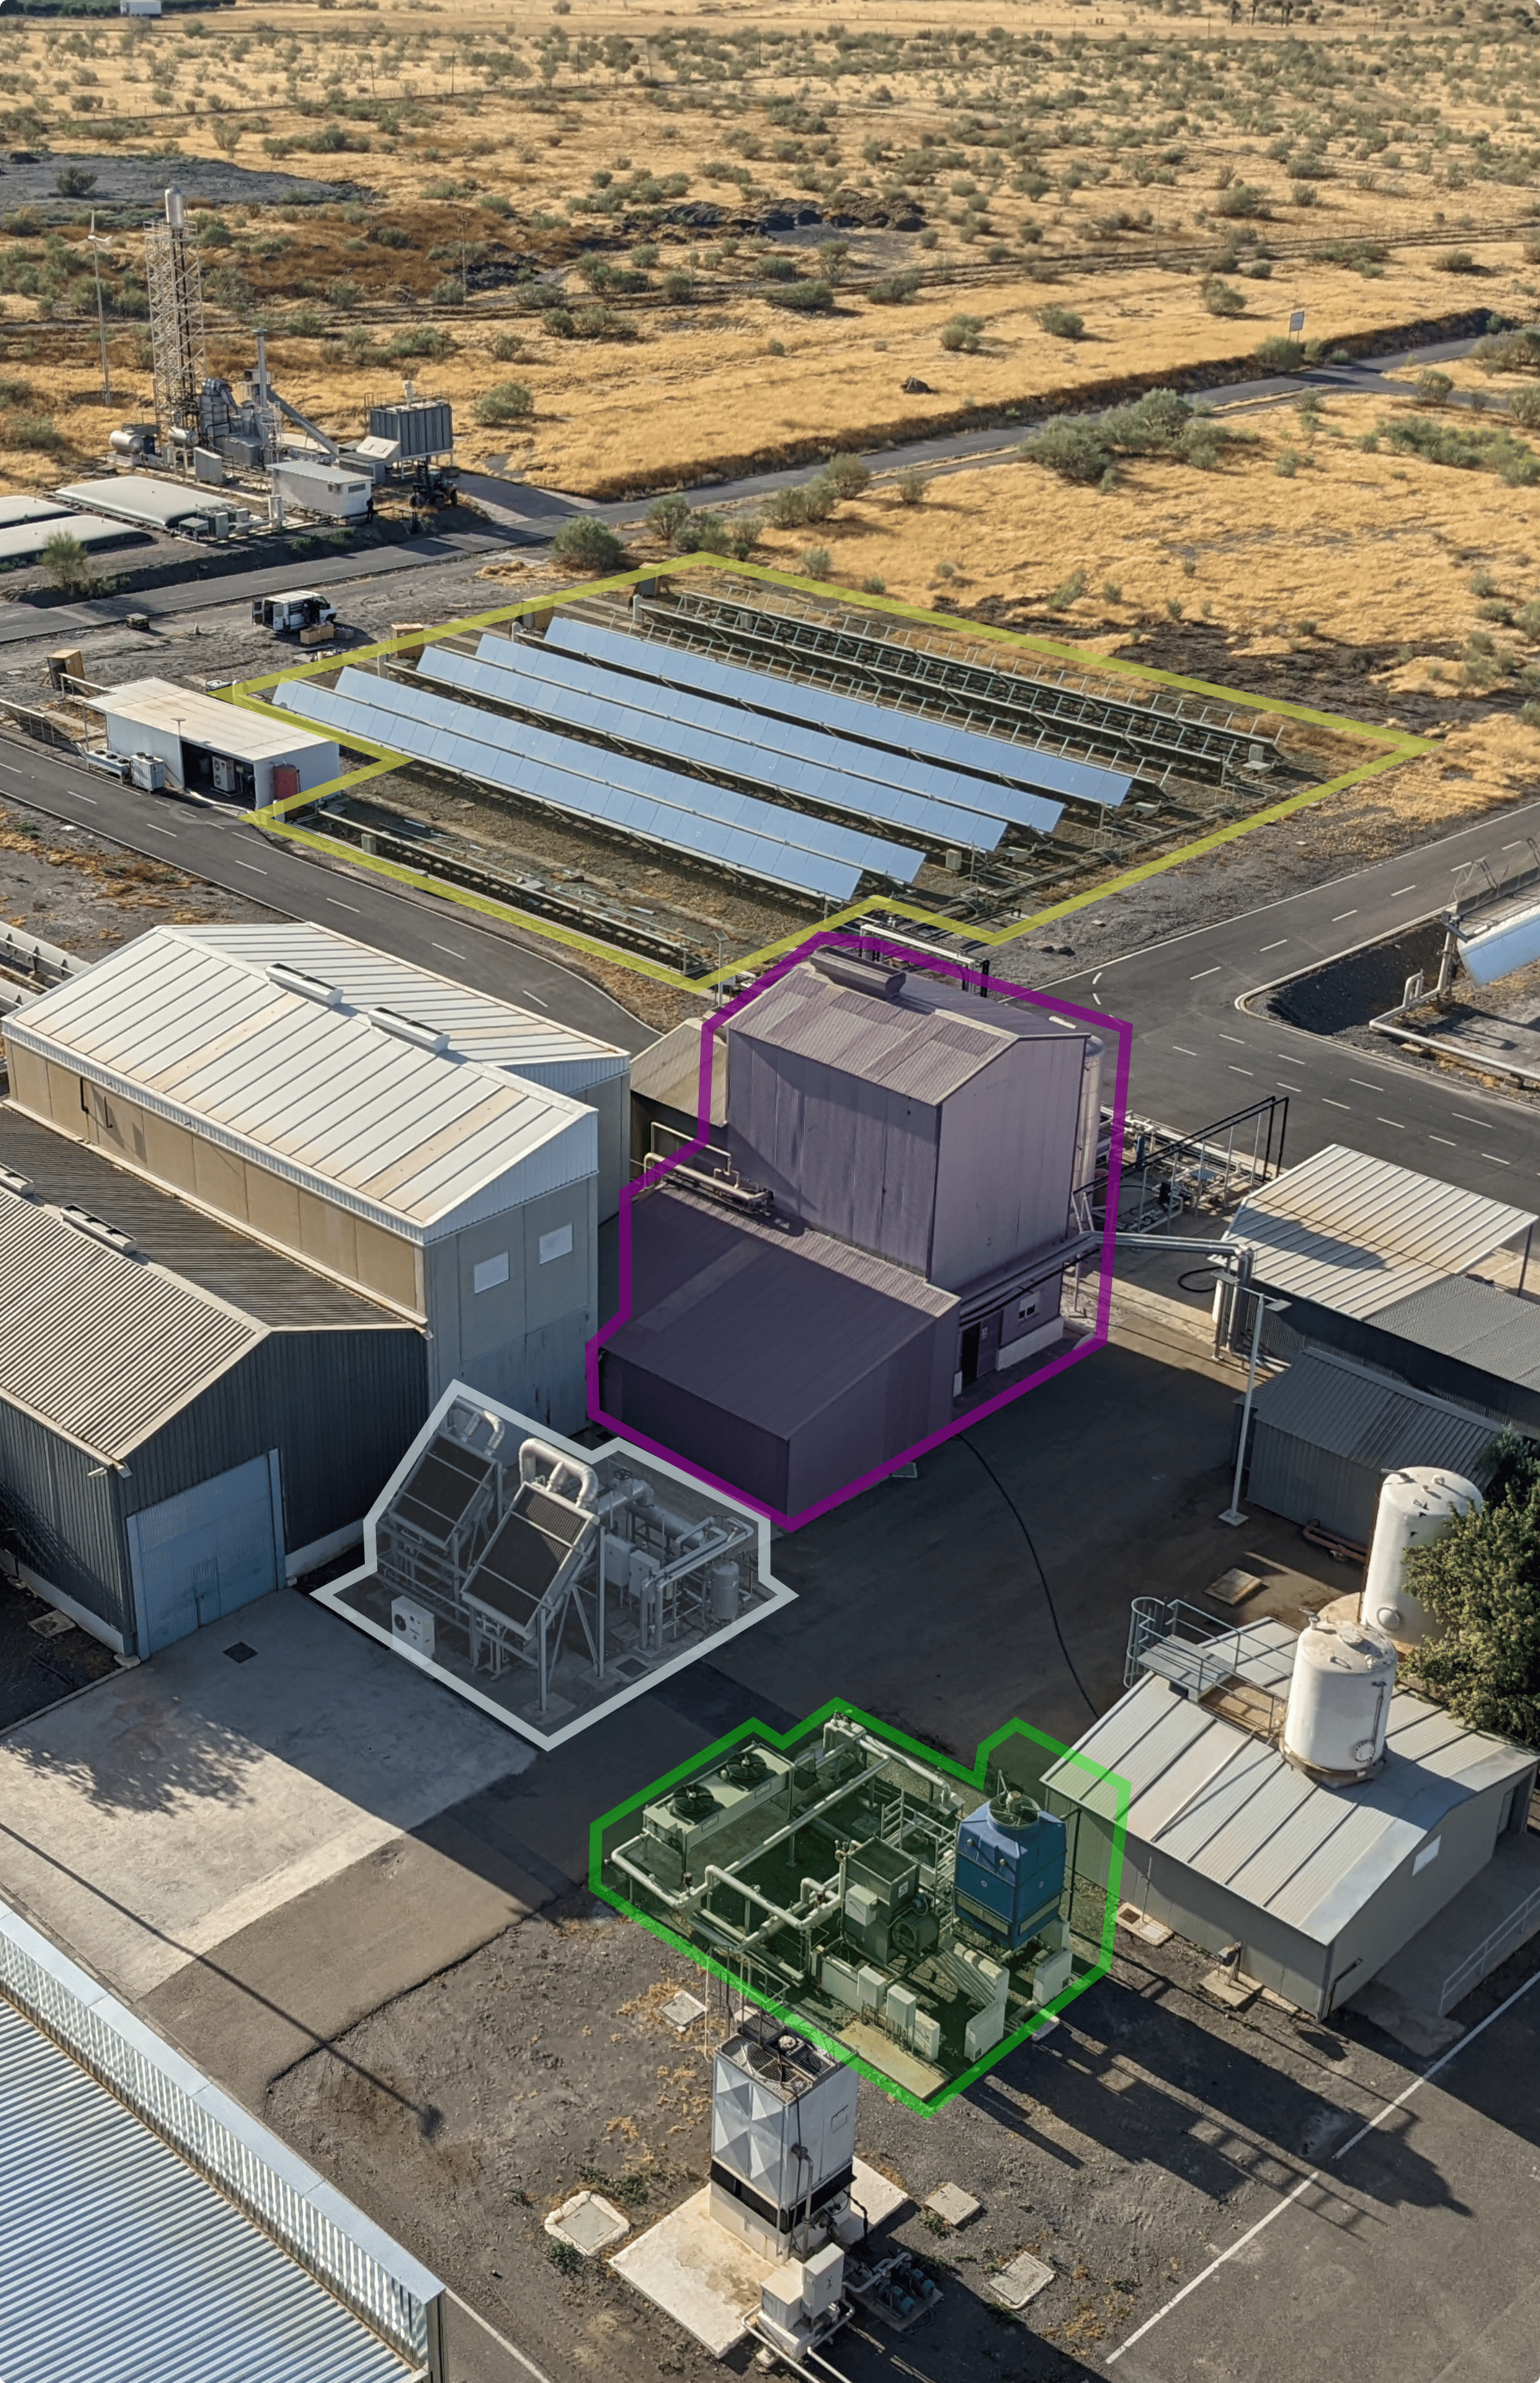
\includegraphics[width=\textwidth]{figures/pilot-plants-aerial-view.png}
    \caption{
        \textbf{Aerial view of the pilot plants at the \fullgls{psaLabel}, Spain.}\\ 
        The developments presented in this thesis have
        been developed and validated around two test-rigs: a
        \gls{ccsLabel} and a \gls{solarmedLabel} pilot plants. In the picture, the
        \gls{ccsLabel} plant is located on the left side, and the...
    }
    \labfig{intro:pilot-plants}
\end{figure}


%===================================
%===================================
%===================================
\setchapterpreamble[u]{\margintoc}
\chapter{Research plan}
\labch{intro:plan}
% Fijarse en Tesis Simon

asdad

%===================================
%===================================
\section{Hypothesis}
\labsec{intro:research-plan:hypothesis}

%===================================
%===================================
\section{Objectives}
\labsec{intro:research-plan:objectives}

%===================================
%===================================
\section{Contributions}
\labsec{intro:research-plan:contributions}


% %===================================
% %===================================
% %===================================
% \setchapterpreamble[u]{\margintoc}
% \chapter{Contributions}
% \labch{intro:contributions}

% % Generales de la tesis, abstracto
% asdad
